\documentclass{article}

\usepackage{graphicx}
%\usepackage{cite}
\usepackage{wrapfig}
\usepackage{placeins}
%\usepackage{biblatex}
\usepackage{hyperref}
\usepackage{indentfirst}
\usepackage[english]{babel}
\usepackage[utf8]{inputenc}
\usepackage{fancyhdr}
\usepackage{csquotes}
\usepackage{multirow}
\usepackage{graphicx}
\usepackage{float}
\usepackage{geometry}

\pagestyle{fancy}
\fancyhf{}
\lhead{Pinball}
\rfoot{Page \thepage}
\lfoot{Software Requirments Specification}

\begin{document}
    \begin{titlepage}
    \begin{center}
        \vspace*{1cm}
        
        \Huge
        \textbf{Pinball}
        
        \vspace{1.5cm}
        \LARGE
        Software Requirments Specification
        
        \vspace{0.5cm}
        \textbf{Version 1.0}

        \vspace{0.5cm}
        \textbf{21-10-2015}

        \vspace{1.5cm}
        \textbf{Group 21}\\
        \textbf{The Pirates}
        
        \vfill
        
        \vspace{0.8cm}        
        \Large
        Prepared for\\
        CS 251 – Software Systems Lab\\
        Instructor: Sharath Chandran\\
        Autumn 2015
        
    \end{center}
\end{titlepage}
    \tableofcontents
    \thispagestyle{empty}
    \cleardoublepage
    \pagenumbering{arabic}
    \newpage

    \section{Introduction}
    The purpose of this document is to present a detailed description of the Web Publishing System. It will explain the purpose and features of the system, the interfaces of the system, what the system will do, the constraints under which it must operate and how the system will react to external stimuli.  This document is intended to contain all of the information needed by a software engineer to adequately design and implement the game of pinball.

    \subsection{Purpose}
    The game is designed as a part of the first project involving box2d for CS251.
    \subsection{Scope}
    The scope of the project is to turn the age old implementation of the arcade pinball game into a computer based game using box2d physics engine. The game is made cross-platform by the use of cmake.
    \subsection{Definitions, Acronyms, and Abbreviations}
    
    \textbf{Flipper Wheel}

    \begin{minipage}[t]{0.6 \textwidth}
        \vspace{0pt}
        Rotating wheel hinged about it’s center.
    \end{minipage}
    \begin{minipage}[t]{0.25\textwidth}
        \vspace{0pt}
        \centering
        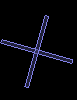
\includegraphics[width=0.9\linewidth,natwidth=610,natheight=642]{flipperWheel.png} 
        \label{fig:flipperWheel}
    \end{minipage}

    \textbf{Sling Shot}

    \begin{minipage}[t]{0.25\textwidth}
        \vspace{0pt}
        \centering
        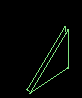
\includegraphics[width=0.9\linewidth,natwidth=610,natheight=642]{slingshot.png} 
        \label{fig:slingshot}
    \end{minipage}
    \begin{minipage}[t]{0.6\textwidth}
        \vspace{0pt}
        Elastic triangular objects.
    \end{minipage}

    \textbf{Flipper Bats}

    \begin{minipage}[t]{0.6\textwidth}
        \vspace{0pt}
        A tapered object that forms the primary means of hitting the ball
    \end{minipage}
    \begin{minipage}[t]{0.25\textwidth}
        \vspace{0pt}
        \centering
        
\includegraphics[width=0.9\linewidth,natwidth=610,natheight=642]{flippers.png} 
        \label{fig:flippers}
    \end{minipage}

    \textbf{Ball}

    \begin{minipage}[t]{0.25\textwidth}
        \vspace{0pt}
        \centering
        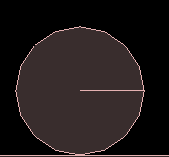
\includegraphics[width=0.9\linewidth,natwidth=610,natheight=642]{ball.png} 
        \label{fig:ball}
    \end{minipage}
    \begin{minipage}[t]{0.6\textwidth}
        \vspace{0pt}
        The circular object that moves around the board
    \end{minipage}
    
    \textbf{Launcher}

    \begin{minipage}[t]{0.6\textwidth}
        \vspace{0pt}
        Provides the initial momentum to the ball propelling it upward.
    \end{minipage}
    \begin{minipage}[t]{0.25\textwidth}
        \vspace{0pt}
        \centering
        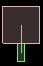
\includegraphics[width=0.9\linewidth,natwidth=610,natheight=642]{launcher.png} 
        \label{fig:launcher}
    \end{minipage}

    \textbf{Bumpers}

    \begin{minipage}[t]{0.25\textwidth}
        \vspace{0pt}
        \centering
        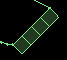
\includegraphics[width=0.9\linewidth,natwidth=610,natheight=642]{bumpers.png} 
        \label{fig:bumpers}
    \end{minipage}
    \begin{minipage}[t]{0.6\textwidth}
        \vspace{0pt}
        Rectangular reflectors from which the ball bounces of.
    \end{minipage}

    \textbf{Shooting Bumpers}

    \begin{minipage}[t]{0.6\textwidth}
        \vspace{0pt}
        Circular objects from which the balls bounce off.
    \end{minipage}
    \begin{minipage}[t]{0.25\textwidth}
        \vspace{0pt}
        \centering
        
\includegraphics[width=0.9\linewidth,natwidth=610,natheight=642]{shootingbumpers.png} 
        \label{fig:shootingbumpers}
    \end{minipage}

    \textbf{Rotators}

    \begin{minipage}[t]{0.25\textwidth}
        \vspace{0pt}
        \centering
        
\includegraphics[width=0.9\linewidth,natwidth=610,natheight=642]{rotators.png} 
        \label{fig:rotators}
    \end{minipage}
    \begin{minipage}[t]{0.6\textwidth}
        \vspace{0pt}
        Continuously rotate in either one of the directions.
    \end{minipage}

    \subsection{References}
    ~\cite{gprof}    
    ~\cite{stack}
    ~\cite{Adit}
    ~\cite{cocos2d}
    ~\cite{iforce}

    \bibliography{report}{}
    \bibliographystyle{plain}

    \subsection{Overview}
    In this report we have given a gist of our design, its salient features and working parts.
    The next sections consists of a general discussion about our project as well as the product functions.

    \section{General Description}
    \subsection{Product Perspective}
    Pinball was first designed as an arcade game in the 19th century. With the advent of the computers the game was also implemented as a computer game. We intend to develop our own version of the game.

    \subsection{Product Functions}
    The major game functions are:\\
    \begin{quote}
    \begin{tabular}{ll}
        Launching the ball&The ball is launched on user giving the command.\\
        Flipper movement&The corresponding flippers are moved based on user input.\\
        Rotate wheels&The direction of rotation of the wheels is changed based on user input.\\
        Restart&The game is to be restarted whenever the user deems right by taking in input.\\
        Pause&Pause the game whenever commanded to.
    \end{tabular}
    \end{quote}

    \subsection{User Characteristics}
    The user is expected to know the controls of the game, how to operate the keyboard and Ubuntu literate in the sense that he knows how to run the game from the terminal using the bash script provided (or otherwise).

    \subsection{Assumptions and Dependencies}
    A) Asssumptions\\

    We assume that the user will restart the game whenever he deems right.\\

    B) Dependencies\\
    
    The speed of execution depends on the processor speed in which the game is being played.

    \section{Specific Requirements}

    \subsection{External Interface Requirements}

    \subsubsection{User Interfaces}

    \begin{minipage}[h]{0.25\textwidth}
        \vspace{0pt}
        \centering
        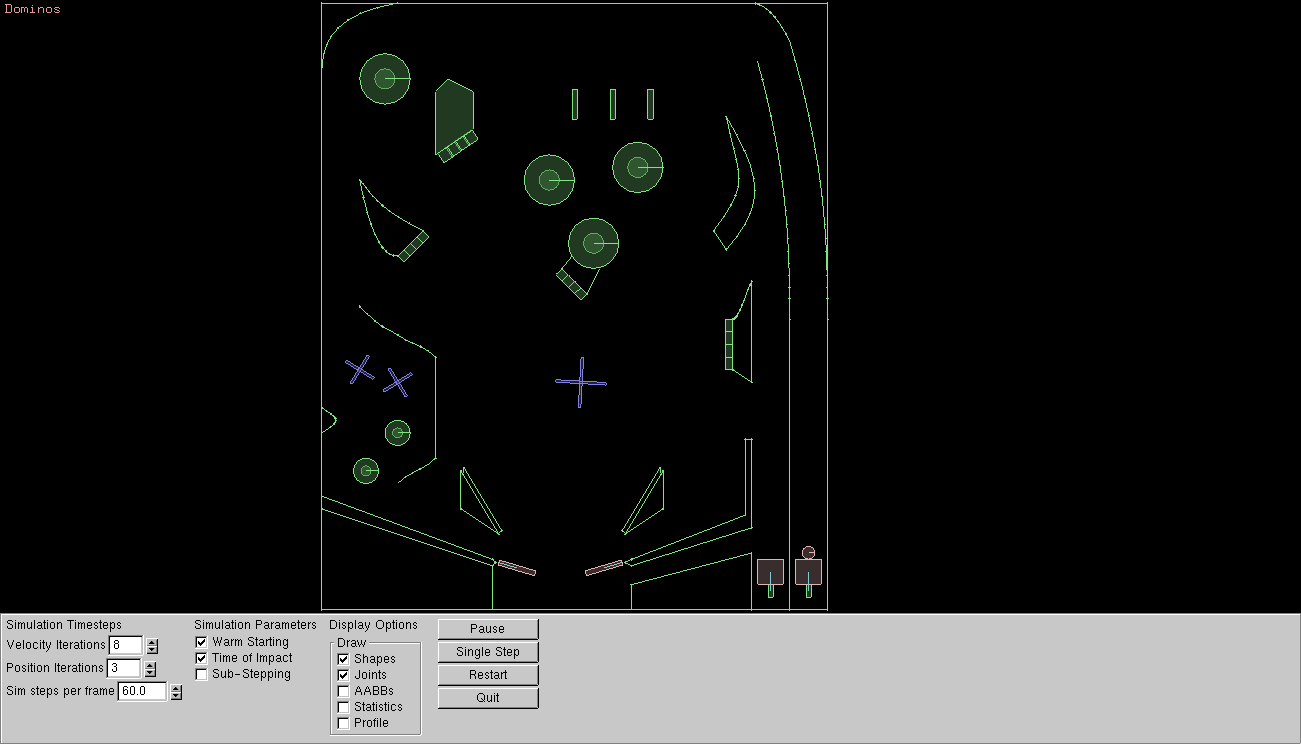
\includegraphics[width=3.5in,natwidth=610,natheight=642]{userInterface.png}
        \label{fig:Pinball}
    \end{minipage}

    \subsubsection{Hardware Interfaces}
    A working keyboard is sufficient to interact with  the game.

    \subsubsection{Software Interfaces}
    cmake is essential to run the game.
    A C++ compiler is also necessary to create an executable for the game.

    \subsection{Functional Requirements}
    On button press:\\
    \begin{quote}
    \begin{tabular}{ll}
        W   :&The launcher on the right is activated and gives a push to the ball.\\
        A   :&The lift flipper turns anti clockwise.\\
        D   :&The right flipper turns clockwise.\\
        R   :&The game is restarted from the start.\\
        P   :&The game is frozen in its current state.\\
        esc :&Quit game console.\\
        8   :&The launcher on the left is activated.\\
        4   :&Change the direction of flipper wheel to counter clockwise.\\
        6   :&Change the direction of flipper wheel to clockwise.
    \end{tabular}
    \end{quote}

    \section{Analysis Models}
    \subsection{Call Graph}

    \begin{minipage}[h]{0.25\textwidth}
        \vspace{0pt}
        \centering
        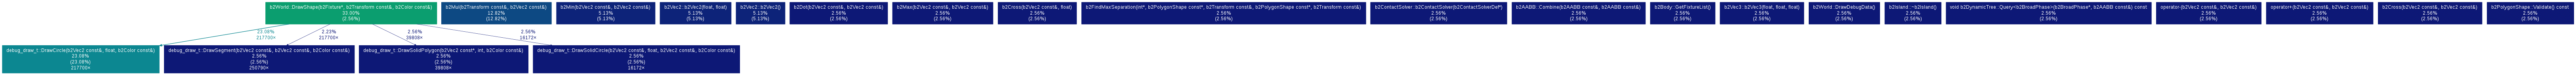
\includegraphics[width=6.5in,natwidth=610,natheight=642]{analysis.png}
        \label{fig:Pinball}
    \end{minipage}

    \section{Revision History}
    %\textbf{Revision History}
    \begin{quote}
        \begin{tabular}{ |c|c|c|c| }
         \hline
         \textbf{Date}&\textbf{Description}&\textbf{Author}&\textbf{Comments}\\
         \hline 
          17-10-2015& Draft of SRS & Sai Teja & Revision Done\\
         \hline 
          19-10-2015& Added images & Chanukya & Revision Done\\
         \hline 
          20-10-2015& Webpage & Naveen & Revision Done\\
         \hline
        \end{tabular}
    \end{quote}

    \section{Document Approval}
    %\textbf{Document Approval}\\

    The following Software Requirements Specification has been accepted and approved by the following:
    \begin{quote}
        \begin{tabular}{ |c|c|c|c| }
         \hline
         \textbf{Signature}&\textbf{Printed Name}&\textbf{Title}&\textbf{Date}\\
         \hline 
          & Prof. Sharat Chandran & Instructor, CS 251 &\\
         \hline
        \end{tabular}
    \end{quote}

    \section{Deviations from ideal}
    \begin{minipage}[t]{0.25\textwidth}
        \vspace{0pt}
        \centering
        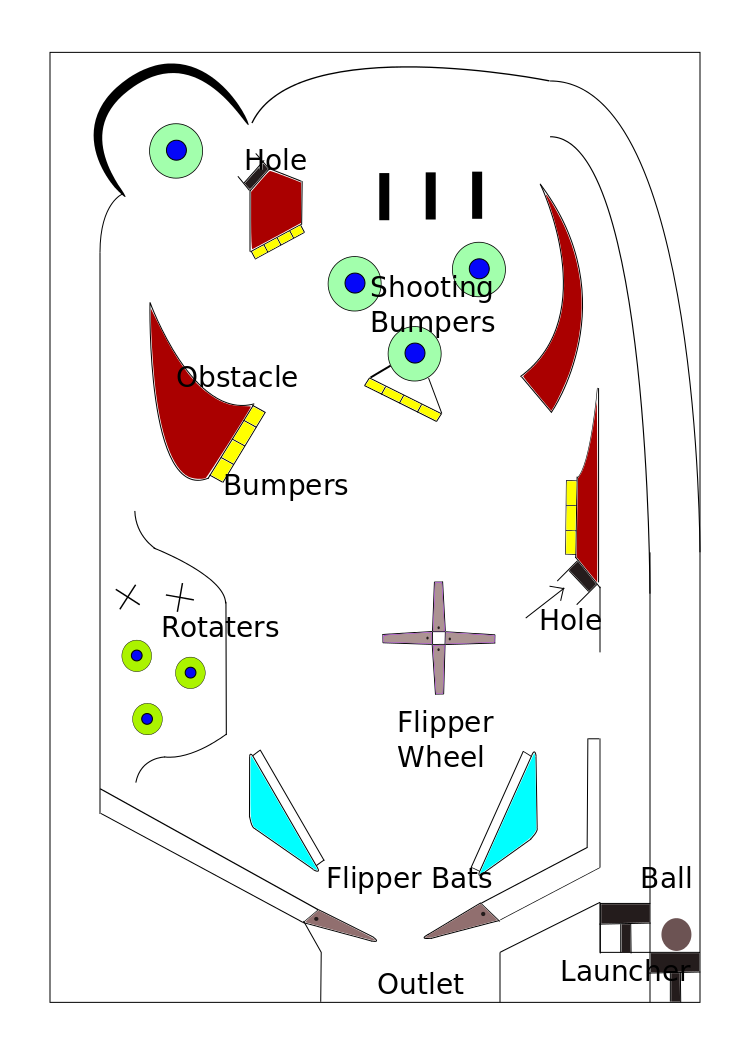
\includegraphics[width=3.5in,natwidth=610,natheight=642]{pinball.png}
        \label{fig:Pinball}
    \end{minipage}
    \hspace{5cm}
    \begin{minipage}[t]{0.25\textwidth}
        \vspace{0pt}
        \centering
        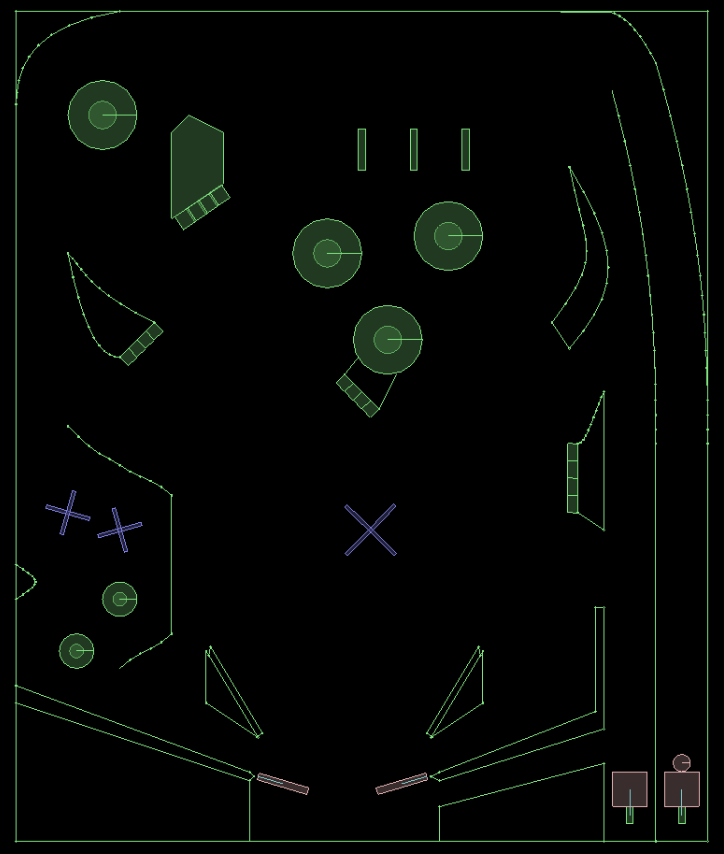
\includegraphics[width=3.5in,natwidth=610,natheight=642]{final.png}
        \label{fig:Pinball}
    \end{minipage}

    \noindent The first figure shows the initial design that we thought of creating for our project.\\
    The second figure shows the final design that we created.\\
    We were not able to create a hole as we were not able to detect collisions.

    \section{Difficulties}
    \noindent We faced some difficulties in giving the keyboard functions to the flipper bats and launcher.\\
    We overcame this problem by using an extern variable so that it can be used over different files and at desired locations.

    \section{Honor Code}
    We pledge on our honor that we have not given or received any unauthorized assistance on this project.

\end{document}